\section{Reproducible software interface}\label{sec:software}
The \texttt{trendestimation} Python package exposes the difference
order, a prescribed difference reference mean, and the normalized
smoothness coordinate. A fitted trend can be selected using the
profiled Gaussian contrast likelihood derived in
Theorem~\ref{thm:reml}. For a previously loaded observation
vector \texttt{y} and a fixed numeric reference \texttt{mu}:

\begin{verbatim}
import numpy as np
from trendestimation import TrendSmoother, select_lambda

solver = TrendSmoother(len(y), order=3)
s_grid = np.linspace(0.02, 0.98, 91)
choice = select_lambda(
    solver, y, criterion="mle", mu=mu,
    search_space="smoothness", grid=s_grid
)
trend = solver.fit(
    y, lambda_=choice.lambda_, mu=mu
).trend
\end{verbatim}

\begin{figure}[H]
\centering
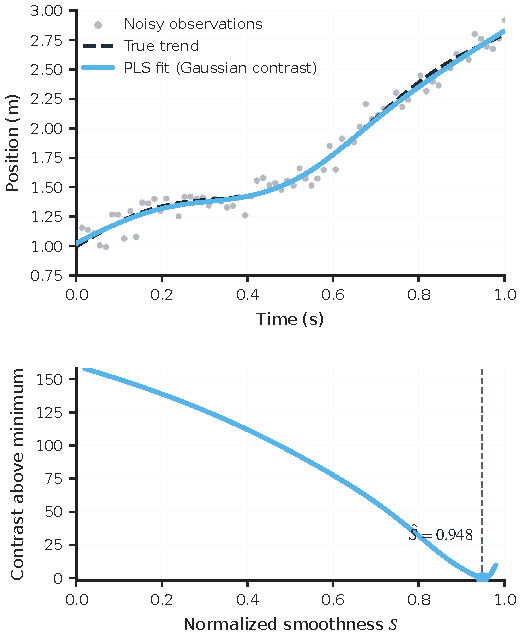
\includegraphics[width=0.98\columnwidth]{figures/gaussian_jerk_demo.pdf}
\caption{A single illustrative third-order PLS fit selected by the
profiled Gaussian contrast likelihood. \emph{Top:} a simulated
position series with independent Gaussian observation noise,
its known cubic-plus-sinusoidal true trend, and the estimated trend.
The cubic baseline corresponds to constant jerk
$1.8\,\mathrm{m\,s^{-3}}$; the added sinusoid produces modest
time-varying jerk. The reference $\mu=1.8h^3$ is fixed from
the known baseline at sampling interval $h$, not estimated
from the observations. \emph{Bottom:} the Gaussian contrast
relative to its smallest evaluated value, plotted against the
normalized smoothness index; the marked $\widehat S$ is the
minimum over 91 predeclared candidates in $[0.02,0.98]$.
This is an in-sample synthetic demonstration, not a
forecasting or comparative-performance experiment.}
\label{fig:gaussian-jerk-demo}
\end{figure}

Figure~\ref{fig:gaussian-jerk-demo} shows what the code returns:
one fitted series and the corresponding selection criterion.
The published example is reproduced with
\texttt{figures/render\_gaussian\_jerk.py}, using the
pinned AwesomeFigures library and a fixed random seed.
The position observations are simulated; no external data
are required, and the same $S$ grid and conditional
fixed-$\mu$ criterion are used in the code and plot.

The interface distinguishes specifying a penalty, requesting a
normalized smoothness level and selecting a candidate by a
statistical criterion. Selection on a finite $S$ grid is
not a certified global continuous optimum. A data-derived
reference \texttt{mu="data"} is a conditional plug-in
and is not the joint unknown-mean REML model proved here.

\paragraph{Reproducibility of the theory.}
The repository retains the deterministic matrix-identity
checks, source data for this example, figure renderer
and numerical validation scripts. No previously recorded
benchmarks are rerun by this demonstration.
